\documentclass{article}
\PassOptionsToPackage{numbers,compress}{natbib}
\usepackage[main]{neurips_2026}

\usepackage[utf8]{inputenc}
\usepackage[T1]{fontenc}
\usepackage{amsmath,amssymb,amsthm,mathtools}
\usepackage{booktabs}
\usepackage{graphicx}
\usepackage{microtype}
\usepackage{xcolor}
\usepackage{hyperref}
\usepackage{url}
\hypersetup{colorlinks=true,linkcolor=blue,citecolor=blue,urlcolor=blue}

\newtheorem{theorem}{Theorem}
\newtheorem{lemma}[theorem]{Lemma}
\newtheorem{proposition}[theorem]{Proposition}
\newtheorem{corollary}[theorem]{Corollary}
\newtheorem{definition}{Definition}
\newtheorem{assumption}{Assumption}
\newcommand{\cA}{\mathcal A}
\newcommand{\cC}{\mathcal C}
\newcommand{\cH}{\mathcal H}
\newcommand{\cO}{\mathcal O}
\newcommand{\Prb}{\mathbb P}
\newcommand{\eps}{\varepsilon}
\DeclareMathOperator{\TV}{TV}

\title{Finite-Sample Recovery of Predictive History Quotients\\from Independent POMDP Trajectories}
\author{Anonymous Authors}

\begin{document}
\maketitle

\begin{abstract}
We study a modest but identifiable abstraction problem for partially observed
control: under one fixed data-collection policy, which bounded observation
contexts have the same finite-horizon continuation law?  We define the
\emph{episode-position predictive quotient}, an explicitly policy- and
position-dependent estimand.  Our estimator first selects contexts on one
half of independently reset trajectories, then takes at most one prespecified
continuation block from each trajectory in the other half.  It compares fixed-
alphabet histograms by empirical total variation and abstains whenever a pair
lacks the samples required by its own concentration bound.  Under an
$\eps$-gap, a per-context visitation floor, and a selection threshold no
larger than the inference threshold, we prove exact recovery with
probability $1-\delta$ from
$O((d+\log(K/\delta))/(\mu_{\min}\eps^2))$ trajectories, where $d$ is the
continuation-alphabet size and $K$ the selected context count.  A two-point
construction shows the dependence on $\mu_{\min}$ and $\eps$ is unavoidable;
the dependence on $d$ is not matched and is known to be improvable by
optimal closeness testers.
The guarantee is non-asymptotic: it does not treat overlapping windows as
independent, does not rely on chi-square calibration, and conditions each
context only on its own count, so nested candidate contexts are covered.
Implementation checks on three analytically solvable environments---each
with $\eps$ set below its known gap---recover the exact quotients on all of
20 seeds, including an environment whose quotient requires merging; a
budget sweep shows the power gate degrading through abstention with no
incorrect merge at any budget; and a position-nonstationary chain shows the
overlapping-window mode systematically merging contexts the
episode-position quotient separates.
\end{abstract}

\section{Introduction}

A partially observed agent must often compress its interaction history.  One
data-accessible compression merges histories that predict the same future
observations.  Related ideas underlie probabilistic suffix automata
\citep{ron1996power}, causal-state reconstruction \citep{shalizi2004blind},
predictive state representations \citep{boots2010closing}, and spectral HMM
learning \citep{hsu2012spectral}.  In controlled systems, however, a
continuation distribution also depends on the behavior policy, reset law,
time within an episode, and sampling protocol.  Ignoring any of these turns
a plausible clustering method into an estimator of a different, well-defined
estimand than the one intended --- it answers a different question.

This paper isolates a finite-sample problem for which those choices are
explicit.  We receive independently reset trajectories generated by a fixed
policy.  Before examining their values, we fix one context endpoint $r$ and a
continuation horizon $k$.  A context $h$ is represented by the conditional law
of the $k$ observations following $r$.  Equal laws define a predictive
quotient.  This is not claimed to be a policy-independent POMDP state, a PSR
rank, or the full infinite-future causal-state partition.

The statistical difficulty is not the histogram alone.  Contexts are
data-dependent, rare contexts have low power, and all sliding windows from an
episode are dependent.  Our construction handles the first two directly and
removes the third by restriction:

\begin{enumerate}
  \item candidate contexts are selected on trajectories disjoint from those
  used for inference;
  \item each inference trajectory contributes at most one prespecified block
  --- fixing the endpoint before data collection makes this restriction
  well-defined, at the price of discarding the rest of each trajectory;
  \item an empirical-TV test has an explicit finite-sample error bound that
  conditions each context only on its own count, so nested contexts sharing
  blocks are covered; and
  \item low-count pairs are returned as \textsc{Undetermined}, never merged.
\end{enumerate}

We do not claim to solve dependent-window inference; we identify the
restricted estimand for which elementary tools suffice and then certify that
estimand end to end.  The contribution is threefold: (i) an explicitly
policy- and position-conditional estimand stated with all of its
conditioning and with a precise downstream currency --- merged contexts are
exchangeable for any window-measurable return
(Proposition~\ref{prop:reward}), (ii) an abstaining finite-sample
certificate whose failure mode \emph{under the stated gap model} is refusal
rather than silent merging --- outside the gap model, \textsc{Same} verdicts
carry no certificate, a regime Section~\ref{sec:checks} exhibits directly
--- and (iii) an implementation
whose procedure, constants, and main-table numbers are mechanically checked
against the theorems, including a budget sweep that exercises the abstention
regime, a misspecification probe that realizes the uncertified-merge regime,
and a head-to-head in which the position-pooling scan returns a
systematically wrong merge relative to the episode-position estimand.  Under a fixed policy with identically reset internal state, the
closed-loop observation process is a hidden-Markov process over the latent
state, policy state, and episode position; the theorems are process-level
statements about that reduction, and the control-specific content enters
through the estimand's scope (Appendix~\ref{app:scope}).  Full proofs, edge
cases, and the exact implementation contract appear in the supplement.

\section{Related work}

\paragraph{Predictive partitions of histories.}
Prediction suffix trees learn variable-memory processes by splitting suffixes
whose next-symbol laws differ \citep{ron1996power}; consistent context-tree
and variable-length Markov chain estimators sharpen that line for stationary
sequences \citep{buhlmann1999variable,csiszar2006context}.  Causal states group
histories with identical conditional futures
\citep{crutchfield1989inferring,shalizi2001computational}, and CSSR
reconstructs them for stationary discrete processes \citep{shalizi2004blind};
our quotient is the bounded-context, fixed-position, finite-horizon
analogue of that construction for the closed-loop process; because a bounded
context carries a mixture over the histories it abbreviates, the quotient
neither refines nor is refined by the causal-state partition in general.  The closest algorithmic
ancestor under control is McCallum's utile-distinction and U-Tree line
\citep{mccallum1995instance,mccallum1996reinforcement}, which splits a suffix
tree of action--observation histories in a POMDP using statistical tests on
future quantities; U-Tree's splits are uncalibrated
Kolmogorov--Smirnov decisions on overlapping experience, and later looping
suffix-tree variants inherit the same uncertificated testing
\citep{holmes2006looping}, whereas our test
carries a finite-sample certificate and abstains.  Our target is
deliberately narrower than all of these: bounded contexts and bounded futures
at one episode position under a fixed policy.  In exchange, our statement is
finite-sample, admits controlled trajectories, and includes context
selection and abstention in the theorem.

\paragraph{Distinguishability-based automaton learning.}
The closest guarantee \emph{shape} appears in PDFA learning by state
merging: ALERGIA merges states whose empirical futures agree
\citep{carrasco1994learning}, and PAC analyses recover the automaton exactly
under a state-distinguishability gap --- in $L_\infty$
\citep{clark2004pac} or, sharpest for comparison, variation distance
\citep{palmer2007pac}; \citet{balle2013learning} organize this line.  We
do not claim a new test statistic or a new proof technique: the ingredients
(an $L_1$ deviation bound, a union bound, a gap assumption) are standard,
and where the data \emph{are} generated by a PDFA those algorithms recover
the whole automaton, which our position-by-position partition does not.  The
differences are of target, not of technique, and we state them as such.
(i)~\emph{Realizability.}  The PDFA results assume the sample is drawn from a
(probabilistic) deterministic automaton, so each history determines its
state.  A POMDP or HMM observed through bounded contexts is generally not
such an automaton: a context carries a mixture over the histories it
abbreviates (Tiger's listen contexts are an example, and
Section~\ref{sec:checks} uses a random three-state HMM), and the PDFA
guarantees say nothing about such data, whereas our estimand, the
continuation law of a bounded context at one position, is well defined for
any finite-alphabet closed-loop process.  CSSR is likewise analyzed for
stationary processes with finitely many causal states and is asymptotic
\citep{shalizi2004blind}; ours is a finite-sample statement about a
non-stationary, reset, position-indexed target.
(ii)~\emph{Closed loop.}  The sample is generated under a stated behavior
policy with actions and early termination, and the estimand conditions on
reaching $r+k$ (Appendix~\ref{app:scope} gives the reduction); that
conditioning, and the policy dependence it induces, are part of the object
being certified, not an afterthought.
(iii)~\emph{What is inside the theorem.}  Context selection, the
sample-splitting that makes it legitimate, an explicit executable gate
$m^*$ with constants, and abstention are all inside
Theorems~\ref{thm:pair}--\ref{thm:recovery} (with nested contexts handled by
the one-count conditioning of Lemma~\ref{lem:onecount}, which has no analogue
when automaton states are disjoint events), and a two-point lower bound
(Proposition~\ref{prop:lower}) shows the $\mu_{\min}$ and $\eps$
dependence cannot be removed.  We have not checked that every published PDFA
result lacks some of these features, and make no claim of dominance:
the delta over that line is the estimand and the executable certificate, and
its practical value for downstream use is argued only through
Proposition~\ref{prop:reward}.

\paragraph{State abstraction and equivalence relations.}
Bisimulation quotients and their metrics are the standard equivalence
notions for fully observed MDPs
\citep{givan2003equivalence,ferns2004metrics}, organized into an abstraction
taxonomy by \citet{li2006towards}; \citet{castro2009equivalence} study the
corresponding belief and trace equivalences for POMDPs, fixed-policy
($\pi$-)bisimulation \citep{castro2020scalable} fixes the behavior policy as
we do, and learned bisimulation metrics carry these equivalences into
representation learning \citep{zhang2021learning,castro2021mico}.  In that taxonomy
our estimand is a fixed-policy, observation-only trace equivalence at one
position: in general \emph{incomparable} with belief bisimulation --- it can
merge belief-distinct histories with equal $k$-step futures, and under a
history-dependent policy it can split belief-equal ones
(Appendix~\ref{app:scope}) --- and
preserving conditional return distributions only for window-measurable
rewards (Proposition~\ref{prop:reward}) --- unlike (approximate)
information states \citep{subramanian2022approximate}, which compress
history subject to planning-loss bounds.  We certify recovery of the
partition and its window-return exchangeability, not planning utility.
The nearest recent construction by name is the agent-bounded-indistinguishability
(probe-exact) quotient of \citet{nixon2026myhill}.  As described in its
abstract and main text, it is defined for a known finite POMDP: histories are
merged when no controller in a fixed probe family of finite-state controllers
separates their conditional suffix laws under a closed-loop Wasserstein
pseudometric over a finite horizon, and the paper proves the resulting
quotient canonical, minimal and unique (a bounded-interaction analogue of
Myhill--Nerode), exactly sufficient for observation--action objectives under
clock-aware probes, and approximately sufficient for latent-state rewards.
Its theory is exact and model-based; as far as we can tell from the text we
read, it gives no finite-sample guarantee for learning the quotient from
trajectories, and its sampled experiments are described as exploratory.
Ours is complementary rather than a refinement of it: we take
a \emph{single} behavior policy (a one-element probe family, in that
language) and total variation on a finite alphabet rather than a controller
family and Wasserstein distance, we are indexed by an episode position and
condition on reaching $r+k$, and our contribution is a finite-sample
certificate for estimating that quotient from independently reset
trajectories, which that work does not claim.  We do not prove a formal
refinement or coarsening relation between the two quotients for a given
policy; in particular its canonicity and decision-sufficiency results are
not inherited by ours, and ours does not inherit its probe-family
universality.


\paragraph{Latent-state decoding and PAC POMDP learning.}
Block-MDP and rich-observation methods recover latent state partitions from
trajectories with finite-sample guarantees
\citep{krishnamurthy2016pac,du2019provably,misra2020kinematic}, and
short-term-memory POMDPs formalize when a bounded suffix window suffices
\citep{efroni2022provable}; recent work settles broader learnability
questions for POMDPs and PSRs \citep{liu2022partially,golowich2022learning,
jin2020sample,guo2016pac}.  Those results target model, decoder, or policy
learning under reachability or observability assumptions and typically drive
exploration; we estimate a fixed-policy finite-window partition under a
visitation floor and make no control claim.  PSRs and observable-operator
methods represent predictions of action-conditioned tests through a low-rank
linear state \citep{littman2001predictive,singh2004predictive,
jaeger2000observable,boots2010closing,hsu2012spectral}.  Their rank and our
number of equal closed-loop continuation laws need not order one another; we
therefore make no ``smaller than PSR'' claim.  Neural causal-state
representations learn predictive summaries of action--observation histories
\citep{zhang2019causal}; their focus is representation and downstream
control, whereas ours is an exact finite-alphabet partition with an
abstaining finite-sample certificate.  Model-based lossless history
clustering has been used to accelerate Dec-POMDP planning
\citep{oliehoek2009lossless}; our setting instead learns a policy-specific
predictive partition from sampled trajectories.

\paragraph{Testing and calibration.}
Each pairwise decision is an instance of two-sample closeness testing on a
$d$-element alphabet \citep{batu2000testing}.  Our plug-in TV test pays
$\Theta(d/\eps^2)$ samples per pair; optimal closeness testers achieve
$\Theta(\max(d^{2/3}/\eps^{4/3},\, d^{1/2}/\eps^2))$ \citep{chan2014optimal}.
Corollary~\ref{cor:tester} makes the substitution precise: any closeness
tester replaces the plug-in test inside the same union bound on every pair
of \emph{non-nested} contexts, while nested pairs genuinely require the
one-count conditioning of Lemma~\ref{lem:onecount}; and because published
optimal testers state their complexity only up to unspecified constants,
the substituted gate is no longer a closed-form function of its own bound
(Appendix~\ref{app:tester}).  We retain
the linear-in-$d$ plug-in test on all pairs as the price of an executable
gate; the $d$-dependence of our upper bound
is a design choice, not a proven necessity
(Section~\ref{sec:estimator}).  Classical likelihood-ratio tests use an
asymptotic chi-square calibration.  Our software retains such a G-test for
exploratory analysis, but the theorem-facing path instead uses the
finite-alphabet $L_1$ deviation inequality of \citet{weissman2003l1}.
Sample splitting is classical for making selection compatible with
inference \citep{cox1975note,wasserman2009high} and is what makes the random
context set compatible with a direct union bound here; abstention has a
corresponding tradition in selective classification
\citep{chow1970optimum,elyaniv2010foundations}, though our gate refuses on a
precomputed count threshold, never on the realized statistic --- a power
gate, not a data-adaptive rejector.

\section{Estimand and data contract}

Let $Z_i=(O_{i,0},A_{i,0},O_{i,1},\ldots)$, $i=1,\ldots,N$, be independent
trajectories.  Each trajectory is generated by the same reset distribution
and the same fixed policy $\pi$, whose internal state (if any) is reset
identically.  The policy may depend on within-episode history.  Fix a context
endpoint $r\ge0$, maximum context length $L$, and future horizon $k\ge1$ before
seeing trajectory values.  Only lengths $1\le \ell\le\min(L,r+1)$ are
eligible.  The empty root is excluded throughout.

For $h=(o_{r-\ell+1},\ldots,o_r)$ define the continuation
$C=(O_{r+1},\ldots,O_{r+k})\in\cC=\cO^k$.  A trajectory that terminates before
$r+k$ contributes no block.  Let
\begin{equation}
  P_h(c)=\Prb_\pi(C=c\mid H=h,\; Z\text{ reaches }r+k),
  \qquad c\in\cC.                                      \label{eq:law}
\end{equation}
The conditioning event and its probability are part of the estimand.

\begin{definition}[Episode-position predictive quotient]
For a finite candidate set $\cH$, define $h\sim g$ iff $P_h=P_g$.  The
quotient is $\cH/{\sim}$.  Its visitation mass is
$\mu_h=\Prb(H=h, Z\text{ reaches }r+k)$.
\end{definition}

Because eligible lengths overlap, a realized history at endpoint $r$ matches
up to $\min(L,r+1)$ nested contexts, which the quotient treats as distinct
elements of $\cH$; the induced map from histories to states assigns each
history the class of its longest eligible context, in the manner of suffix-
tree leaf semantics (Appendix~\ref{app:scope}).  Merged contexts are
exchangeable for evaluating any return that is measurable in the
continuation window (Proposition~\ref{prop:reward}).

This equivalence is policy dependent in general: two contexts inducing the
same latent belief can still have different joint action--observation futures
under a history-dependent policy.  If actions are included, the continuation
alphabet is $(\cA\times\cO)^k$ and has size
$|\cA|^k|\cO|^k$, not $|\cO|^k$.  Appendix~\ref{app:scope} states both facts
formally.  For continuous observations, binning defines a new discrete
estimand; it does not automatically recover the unbinned quotient.

\paragraph{Gap model.}
Exact partition recovery is impossible without separation.  We assume that
for every $h,g\in\cH$, either $P_h=P_g$ or
\begin{equation}
  \TV(P_h,P_g)\ge\eps, \qquad \eps\in(0,1].             \label{eq:gap}
\end{equation}
The visitation assumption is per context, $\mu_h\ge\mu_{\min}>0$; class mass
alone is insufficient to ensure samples for every representative.

\section{Estimator}\label{sec:estimator}

Partition trajectory identifiers before collection and split whole trajectories
into a selection half and an inference half (the implementation uses collection
order, fixed independently of trajectory values).  At endpoint
$r$, retain contexts observed at least $q$ times in the selection half, with
$q\le m^*$ for the complexity statement below.  On
the inference half, take at most one block at the same fixed endpoint from
each trajectory.  Let $m_h$ and $\widehat P_h$ be its count and empirical law.

For alphabet size $d=|\cC|$ and pairwise budgets $\alpha,\beta$, define
\begin{equation}
m^*(\eps,\alpha,\beta,d)=
\left\lceil \frac{8}{\eps^2}
\left((d+1)\log2+\log\frac{1}{\alpha\wedge\beta}\right)
\right\rceil .                                        \label{eq:mstar}
\end{equation}
For each pair, return \textsc{Undetermined} if either count is below $m^*$.
Otherwise return \textsc{Same} when
$\TV(\widehat P_h,\widehat P_g)<\eps/2$ and
\textsc{Different} otherwise.  Union--find transmits only \textsc{Same}
edges.  Thus an abstention can over-split the reported graph but can never be
silently interpreted as evidence of equality.  Boundary flags are
operational: a pair of reported classes is flagged iff at least one context
pair straddling the two classes returned \textsc{Undetermined}, so the
reported separation rests in part on an abstention; per-run flag counts
appear in every certified results row (the head-to-head's compact verdict
table, whose certified arm reports zero abstentions, records verdicts
only).  Every selected context is
retained through inference: a context whose count is too small abstains on
all of its pairs; it is never dropped.  (The implementation additionally
enforces a floor of $30$ samples per histogram; since $m^*\ge30$ in every
configuration reported here, the effective gate is $\max(m^*,30)=m^*$.)

\begin{theorem}[Finite-sample pair test]                 \label{thm:pair}
Fix a pair $h,g$ and any $m\ge1$, and let
\begin{equation}
  B(m,d,\eps)=2^{d+1}\exp(-m\eps^2/8).                  \label{eq:bound}
\end{equation}
If $P_h=P_g$, then
$\Prb\{\textnormal{\textsc{Different}},\, m_h\ge m,\, m_g\ge m\}\le
B(m,d,\eps)$.  If $\TV(P_h,P_g)\ge\eps$, the probability of
$\{\textnormal{\textsc{Same}},\, m_h\ge m,\, m_g\ge m\}$ obeys the same
bound.  Consequently, with $m=m^*$, the two error-with-verdict events have
probability at most $\alpha$ and $\beta$, respectively.
\end{theorem}

The proof bounds, for each context separately, the joint event that its
count reaches $m$ \emph{and} its empirical law deviates; conditional on a
context's own count---a symmetric function of the per-trajectory
``contributes to $h$'' indicators alone---its contributing blocks are iid
draws from $P_h$.  No conditioning on the other context's count is ever
used.  This matters because different context lengths at one endpoint are
nested: every trajectory matching a longer context also feeds its shorter
suffixes, so conditioning on both counts jointly would bias the contributing
sample.  See Appendix~\ref{app:pair}.

\begin{theorem}[Exact recovery on a selected set]        \label{thm:recovery}
Condition on any candidate set $\cH$ chosen using only the selection half,
with $K=|\cH|\ge2$.  Set
$\alpha=\beta=\delta/(2K^2)$ and suppose the gap condition~\eqref{eq:gap}
holds.  With probability at least $1-\delta/2$, every pair whose two counts
reach $m^*(\eps,\alpha,\beta,d)$ receives its correct verdict; in
particular, on the event that every inference count is at least $m^*$,
union--find returns exactly $\cH/{\sim}$ and returns no abstentions.
\end{theorem}

\begin{corollary}[Trajectory complexity]                 \label{cor:sample}
Let the two halves each contain $M=\lfloor N/2\rfloor$ trajectories.  Suppose
a deterministic universe of $K$ eligible contexts containing every context
that selection can return satisfies
$\mu_h\ge\mu_{\min}$ and the gap condition.  If
\begin{equation}
 M\ge \max\left\{
 \frac{2q}{\mu_{\min}},
 \frac{2m^*}{\mu_{\min}},
 \frac{8}{\mu_{\min}}\log\frac{4K}{\delta}
 \right\},                                             \label{eq:sample}
\end{equation}
where $m^*$ uses $\delta/(2K^2)$, then all eligible contexts are
selected, no pair abstains, and the exact quotient is returned with
probability at least $1-\delta$.  Since $q\le m^*$ may be assumed, it
follows that $N=O((d+\log(K/\delta))/(\mu_{\min}\eps^2))$.
\end{corollary}

The count terms follow from multiplicative Chernoff bounds for the selection
and inference halves.  Notice what is absent from~\eqref{eq:sample}: trajectory
length does not create extra iid samples because the certified procedure uses
one block per trajectory.

The allocation $\alpha=\beta=\delta/(2K^2)$ is deliberately conservative:
the proof of Theorem~\ref{thm:recovery} spends only $\delta/(4K)$ across
per-context deviation events, so setting the pairwise budget to that
actual total spend --- a relaxation by a factor of $K/2$ --- shrinks $m^*$
by roughly ten percent in the
configurations reported here ($451\to407$ on the 8-cycle sweep).  We keep
the $K^2$ allocation because it certifies each pairwise verdict at level
$\alpha$ individually, which post-hoc inspection of any single pair can
rely on.

\begin{proposition}[Lower bound]                         \label{prop:lower}
For $0<\eps\le1/4$ and $0<\mu\le1/2$, there are two finite-alphabet,
independently reset trajectory models satisfying the data contract, one with
one predictive class and one with two classes separated by $\eps$, such that
any estimator has worst-case partition error at least $3/8$ whenever
$N\le1/(32\mu\eps^2)$.  Thus the dependence on
$1/(\mu_{\min}\eps^2)$ in Corollary~\ref{cor:sample} is unavoidable.
\end{proposition}

The construction has $d=2$, so it says nothing about the linear dependence
on $d$ in~\eqref{eq:mstar}; that factor is a cost of the plug-in test and
is improvable in principle by optimal closeness testers
\citep{chan2014optimal}.  The $\log K$ factor is likewise not matched.

The construction changes a Bernoulli continuation only after a context of
mass $\mu$ and applies Le Cam's two-point method
\citep[Theorem~2.2]{tsybakov2009nonparametric}; the complete calculation is in
Appendix~\ref{app:lower}.

Two extensions come at no cost to the architecture.  First, the pairwise
test is a module:

\begin{corollary}[Tester substitution on non-nested pairs]\label{cor:tester}
Let $A$ be any two-sample closeness tester that, given $m$ iid samples from
each of two laws on $d$ elements, reports \textnormal{\textsc{Same}} under
equality and \textnormal{\textsc{Different}} under $\TV\ge\eps$, each with
error probability at most $\gamma$ whenever $m\ge n(d,\eps,\gamma)$.
Replace the plug-in test by $A$, and the gate by
$n(d,\eps,\delta/(2K^2))$, on every pair of contexts neither of which is a
suffix of the other, retaining the plug-in test and the $m^*$ gate on
nested pairs.  Theorem~\ref{thm:recovery} holds unchanged.  With the tester
of \citet{chan2014optimal} amplified by majority vote,
$n(d,\eps,\gamma)=O\bigl((d^{2/3}/\eps^{4/3}+d^{1/2}/\eps^{2})
\log(1/\gamma)\bigr)$; when $L=1$ no nested pairs exist and the
substitution is total.
\end{corollary}

The non-nested restriction is genuine, not cosmetic: nested contexts share
their contributing blocks verbatim, so a black-box two-sample tester's
independence requirement fails for exactly the pairs whose analysis
motivated Lemma~\ref{lem:onecount}; and the unspecified constants in
optimal testers leave the substituted gate non-executable as a closed-form
abstention rule (Appendix~\ref{app:tester}).

Second, the single endpoint generalizes by one union-bound level:

\begin{corollary}[Multi-endpoint families]\label{cor:multi}
Fix endpoints $r_1<\dots<r_T$ and horizon $k$ before data collection, and
run selection and inference at every endpoint on the same two halves with
per-endpoint failure budget $\delta/T$ (so $\alpha=\beta=\delta/(2TK_t^2)$
at endpoint $r_t$, and the count conditions of Corollary~\ref{cor:sample}
hold with $\delta/T$ in place of $\delta$).  With probability at least
$1-\delta$, every endpoint's quotient is recovered exactly,
simultaneously.  Each trajectory contributes at most one block per
endpoint, no independence across endpoints is used, and the gate grows
additively in $\log T$:
$m^*(\eps,\delta/(2TK_t^2))=\lceil(8/\eps^2)((d+1)\log2+
\log(2TK_t^2/\delta))\rceil$.
\end{corollary}

Proofs are in Appendix~\ref{app:tester}.

\section{Implementation checks}\label{sec:checks}

The repository contains two modes.  The certified mode implements the data
split, fixed endpoint, one block per inference trajectory, fixed alphabet,
TV threshold, Bonferroni budget, and $m^*$ gate above.  A separate exploratory
mode scans overlapping windows and offers chi-square G-tests or kernel tests;
it is not covered by Theorems~\ref{thm:pair}--\ref{thm:recovery}.

Table~\ref{tab:smoke} reports regression checks over 20 seeds per
environment, each with $\eps$ set below the environment's known analytic
gap.  Tiger \citep{cassandra1994acting} uses an always-listen,
history-independent policy, $r=1$,
$k=L=1$, 20{,}000 episodes, selection threshold $q=10$, and $\eps=0.45$; its
two context laws are separated by exactly $(2a-1)^2=0.49$ at listen accuracy
$a=0.85$.  The 8-cycle uses its single action, $r=0$, $k=L=1$, 8{,}000
episodes, $q=100$, and $\eps=0.5$ against an analytic gap of $0.7225$.  The
noisy depth-2 chain exercises the merge path: at $r=0$ and $k=1$ its three
length-one contexts induce exactly two continuation laws (two contexts share
one row of the transition table verbatim), so correct recovery requires a
\textsc{Same} verdict; it uses 16{,}000 episodes, $q=30$, and $\eps=0.5$
against a gap of $0.7524$.  All runs use a 50/50 split and
$\delta=\beta=0.05$.  Recovery is exact on all $3\times20$ runs with no
abstention; the harness fails if any environment's $\eps$ exceeds its
recorded analytic gap.

\begin{table}[t]
  \centering
  \caption{Implementation checks for the certified path, 20 seeds per row.
  ``recovered'' is the class count, identical across seeds (the checker
  fails otherwise); ``Und.'' is the maximum abstaining pair fraction over
  seeds.  Class counts alone do not show that the \emph{partitions} are
  right; Appendix~\ref{app:envs} lists the full transition and observation
  specification of every environment and reports, for every seed, the
  recovered partition and its pair-level error against the exact truth
  (Table~\ref{tab:partitions}).}
  \label{tab:smoke}
  \begin{tabular}{lrrrrr}
    \toprule
    environment & episodes & seeds & expected & recovered & Und.\\
    \midrule
% BEGIN AUTOGEN: independent_smoke
    Tiger (always listen) & 20,000 & 20 & 2 & 2 & 0.00\\
    noisy 8-cycle & 8,000 & 20 & 8 & 8 & 0.00\\
    noisy depth-2 (merge) & 16,000 & 20 & 2 & 2 & 0.00\\
% END AUTOGEN: independent_smoke
    \bottomrule
  \end{tabular}
\end{table}

\begin{figure}[t]
  \centering
  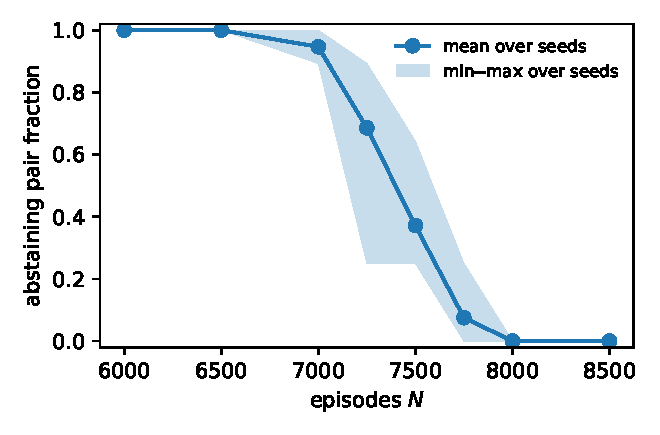
\includegraphics[width=0.62\linewidth]{figures/abstention_sweep.pdf}
  \caption{The power gate binding on the noisy 8-cycle (10 seeds per
  budget).  With $K=8$ contexts, $d=8$, and
  $\alpha_0=\delta/(2K^2)$, the gate requires $m^*=451$ inference samples
  per context; per-context counts at budget $N$ concentrate near $N/16$, so
  abstention collapses from total to zero across
  $N\in[6{,}500,\,8{,}000]$.  At every budget and seed the estimator
  reports all 8 classes---degradation is pure abstention, never an
  incorrect merge.  The main-table budget $N=8{,}000$ sits just above this
  transition.}
  \label{fig:sweep}
\end{figure}

Figure~\ref{fig:sweep} exercises the regime the abstention machinery exists
for: a budget sweep on the 8-cycle in which the $m^*$ gate binds sharply.
Across all 80 sweep runs no class pair is ever merged incorrectly; refusal
is the only failure mode observed, as designed.

\begin{figure}[t]
  \centering
  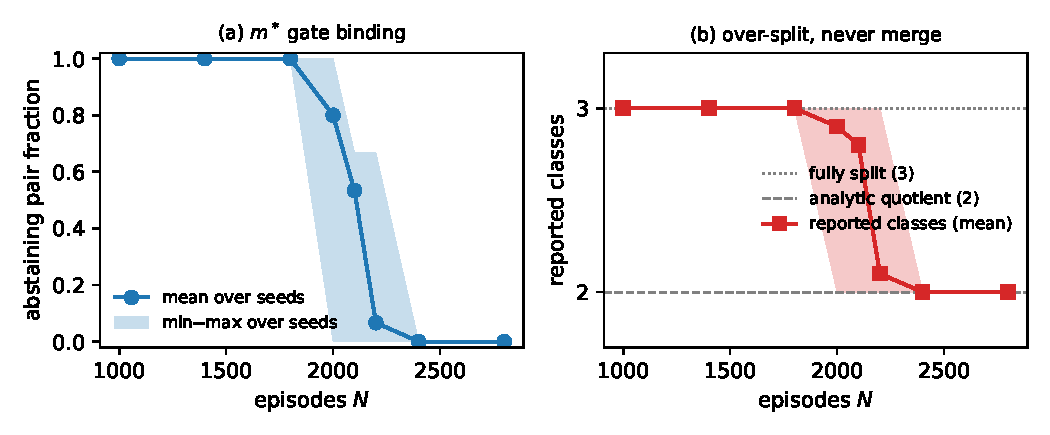
\includegraphics[width=0.9\linewidth]{figures/sweep_depth2.pdf}
  \caption{The same budget sweep on the noisy depth-2 chain at $r=0$,
  whose quotient genuinely merges two of its three contexts (10 seeds per
  budget, $\eps=0.5$ against gap $0.7524$, $m^*=278$).  Below the gate
  transition the required \textsc{Same} verdict abstains and the report
  \emph{over-splits} to three classes; above it the correct two classes are
  reported.  The transition is bracketed in $N\in[2{,}000,\,2{,}400]$,
  matching the prediction $N\approx2{,}050$ from the gate and the
  per-context masses.  Across all 80 runs no pair is merged incorrectly.}
  \label{fig:sweepdepth2}
\end{figure}

The 8-cycle's quotient has no equal pair, so its sweep cannot show what
starvation does to a \emph{merge}.  Figure~\ref{fig:sweepdepth2} repeats
the sweep on the noisy depth-2 chain, where correct recovery requires a
\textsc{Same} verdict: an abstaining gate withholds exactly that verdict,
so degradation appears as over-splitting --- three reported classes instead
of two --- and never as an incorrect merge.  The two sweeps together
exhibit both directions of the refusal semantics.

\paragraph{Nested contexts at $L=2$.}
Every row of Table~\ref{tab:smoke} has $L=1$, where no context is a suffix
of another and the one-count conditioning of Lemma~\ref{lem:onecount} is
never stressed.  A separate check runs the noisy depth-2 chain at endpoint
$r=1$ with $L=2$: twelve eligible contexts (three of length one, each the
suffix of three length-two extensions), an analytic quotient of five
classes, and minimal between-class TV $2/7\approx0.2857$ --- attained by
the \emph{nested} pair $(0,)$ vs.\ $(0,0)$, so the binding decision is one
a black-box two-sample tester could not certify
(Corollary~\ref{cor:tester}).  With $\eps=0.28$, $K=12$, $d=3$, and
$m^*=1{,}167$, the rarest context (mass $\approx0.022$) needs the bulk of
the budget: $140{,}000$ episodes yield roughly $1{,}500$ inference blocks
for it.  Recovery of the five-class nested partition is exact on all 20
seeds with zero abstention.

\paragraph{Head-to-head: pooling positions changes the estimand.}
A binary chain whose transition kernel flips with the parity of the episode
position makes the motivating failure concrete.  At $r=0$ its two length-one
contexts have continuation laws $\mathrm{Ber}(0.9)$ and $\mathrm{Ber}(0.1)$
--- distinct classes at TV $0.8$ --- while every observation is marginally
uniform at every position, so the \emph{position-pooled} continuation law
after either context is exactly $\mathrm{Ber}(0.5)$.  The certified arm
uses 4{,}000 trajectories per seed, selection threshold $q=10$, and
$\eps=0.75$ against the analytic gap $0.8$; the exploratory arm scans
overlapping windows on 400 trajectories of length up to 40, giving it
several times \emph{more} raw windows than the certified arm has blocks
--- an imbalance favoring the exploratory arm.  On 10 seeds each, the
certified path at $r=0$ recovers the two classes with no abstentions in
10/10 runs, while the exploratory overlapping-window mode merges the pair
in 10/10 runs; because the pooled law is exactly $\mathrm{Ber}(0.5)$, that
merge is budget-independent.  The exploratory merge is not a calibration accident and
does not vanish with more data: the scan consistently estimates the pooled
law, a different estimand under which the merge is correct.  This is
precisely the sense in which an unstated sampling protocol turns a
plausible clustering into an estimator of a different estimand than the one
intended (Section~1).  The exploratory arm is our own implementation of
representative overlapping-window practice, labeled as such: we are not
aware of a published
implementation that instantiates the episode-position estimand (fixed endpoint,
termination conditioning, one block per trajectory), so the comparison
available on this target is against practice, not against a published
system.

\paragraph{Two endpoints at once.}
The position-flip chain also instantiates Corollary~\ref{cor:multi} at
$T=2$: its parity-flipped kernel gives two endpoints $r\in\{0,1\}$ with
analytic gap $0.8$ at each.  One shared pool of $4{,}000$ trajectories per
seed is processed at both endpoints on the same two halves, with the family
budget split as $\delta/2$ per endpoint ($\eps=0.75$, $m^*=112$).  Both
endpoint quotients are recovered exactly and simultaneously on 10/10 seeds
with zero abstention --- long trajectories reused across endpoints at
union-bound cost, no mixing argument.

\paragraph{A nondegenerate stochastic policy.}
Every row above fixes a degenerate policy (Tiger's always-listen, the
cycles' single action).  Rerunning Tiger at $r=1$, $k=1$ under the
memoryless stochastic policy (listen $0.8$, open either door $0.1$ each)
exercises the closed-loop framing.  The timeline matters.  The reset emits
an uninformative $O_0$; action $A_0$ emits $O_1$, the context; action
$A_1$ emits $O_2$, the continuation.  A door opening ends the episode, but
the uniform terminal draw it emits \emph{is recorded} as that step's
observation.  Hence the trajectory reaches $r+k=2$ if and only if
$A_0=\textsc{listen}$ (probability $p_\ell=0.8$); if $A_0$ opens a door,
$O_1$ is recorded but no $O_2$ exists and the trajectory contributes no
block.  $A_1$ is unrestricted: with probability $p_\ell$ it is a listen
and $O_2$ is the accuracy-$a$ draw ($a=0.85$), with probability $1-p_\ell$
it is a door opening and the recorded $O_2$ is uniform.  Since the tiger
state is fixed within the episode and $O_0$ is uninformative, conditioning
on $\{O_1=\text{left},\ \text{reach}\}$ multiplies the prior $1/2$ by
$p_\ell\,a$ for tiger-left and $p_\ell(1-a)$ for tiger-right, so
\[
  P_{\text{left}}(O_2{=}\text{left})
  = p_\ell\bigl(a^2+(1-a)^2\bigr)+\tfrac{1-p_\ell}{2}=0.696,\qquad
  P_{\text{right}}(O_2{=}\text{left})
  = p_\ell\,2a(1-a)+\tfrac{1-p_\ell}{2}=0.304 ,
\]
and the survival factor $p_\ell$ from $A_0$ cancels, because it multiplies
numerator and normalizer alike (each context has mass $\mu_h=p_\ell/2=0.4$).
The gap is therefore $\TV=p_\ell\,(2a-1)^2=0.8\cdot0.49=0.392$: the
always-listen gap shrunk by the probability that the \emph{second} action
$A_1$ is informative, not by the reaching event.  Three computations agree
on these numbers: this closed form, an exhaustive enumeration of the latent
chain, and a $400{,}000$-episode Monte Carlo through the collection
code (reach fraction $0.8006$; $0.698$ and $0.305$ for the two
conditional laws; $\TV=0.393$; \texttt{check\_tiger\_stochastic.py}).
With $\eps=0.35$ (checked at runtime against the enumerated gap) and
$8{,}000$ episodes, recovery against the enumerated ground truth is exact
on 20/20 seeds with zero abstention, with $1{,}548$--$1{,}619$ inference
blocks in the rarer context (per seed) against $m^*=468$.  (Writing this check exposed a
seeding defect in the collection routine: the policy generator shared its
seed with the environment's, coupling action draws to Tiger's noise, so
that the sampled stochastic-policy process had conditional laws $0.78$ and
$0.22$ rather than the enumerated ones.  The generators are now independent,
a unit test pins the conditional law, and this check and its artifacts were
regenerated after the fix; the other rows use a single action or a constant
policy, whose actions cannot interact with the environment's noise.)

\paragraph{A data-driven $\eps$: a diagnostic, not a certificate.}
Every configuration so far sets $\eps$ below a gap known by construction.
This last positive check leaves that regime, but it carries \emph{no
certificate}, and we do not count it as evidence for
Theorem~\ref{thm:recovery}.  The environment is a randomly parameterized
three-state HMM whose instance was selected by a rule fixed before any
estimator output (first Dirichlet draw with brute-force minimum pairwise TV
at least $0.15$; the draw used has true minimum TV $0.3872$, computed only
post hoc from the drawn matrices), and $\eps$ is not supplied analytically:
on the \emph{selection half only}, the pairwise empirical-TV spectrum is
sorted with $0$ prepended, and $\widehat\eps$ is the midpoint of the largest
gap whose lower edge lies below $0.5$, with an abstain-on-all-pairs fallback
if that gap is smaller than $0.1$.  Because $\widehat\eps$ and the candidate
set depend on the selection half alone, the inference half is independent of
them, so conditionally on the selection half the pair test is exactly the
fixed-$\eps$ test of Theorem~\ref{thm:pair} run at $\eps=\widehat\eps$.  The
theorem's conclusion, however, needs $\widehat\eps$ to satisfy the gap
model~\eqref{eq:gap}, that is, $\widehat\eps\le$ the true minimum TV
(and distinct classes at least $\widehat\eps$ apart), and nothing in the
paper bounds the probability that the recipe overshoots: the spectrum rule is
a heuristic, and a certification argument would need a selection-half
lower confidence bound on the minimum gap, which we do not provide.  The
check that $\widehat\eps\le0.3872$ uses the true minimum TV, which a user
would not have; it is a post hoc diagnostic of this one instance, not
something the procedure can verify.  What the run shows is limited
accordingly: over 20 seeds at $30{,}000$ episodes no fallback fired,
$\widehat\eps\in[0.189,0.199]$ (all below the post hoc $0.3872$, so none
violated the gap model here), and the three-class truth was recovered
exactly on 20/20 seeds with zero abstention.  We make no claim about how
often the recipe is valid on other instances.

\paragraph{Misspecification probe: the regime outside the gap model.}
The gap model is an assumption, and Section~\ref{sec:estimator}'s refusal
semantics do not survive its failure; one check realizes that failure
deliberately rather than leaving it hypothetical.  A three-context chain is
engineered with one pair at true TV $0.1$ and the others at $0.8$, and the
certified machinery is run verbatim with $\eps=0.5$ --- above the sub-gap
pair's true distance, violating~\eqref{eq:gap}.  On 10/10 seeds the
sub-gap pair is silently merged under a confident \textsc{Same} verdict:
no abstention (the $m^*$ gate is comfortably passed), and no near-threshold
flag (the per-pair artifact records every \textsc{Same} edge's TV margin to
the threshold; the rule margin $<\eps/8$ never fires, mean margin $0.14$).  The separated pairs
are all classified correctly; the report deletes one class.  The honest
price of resolving the engineered pair is stated by the theory itself:
$\eps=0.1$ requires $m^*=6{,}927$ blocks per context, roughly
$42{,}000$ episodes at this layout versus the $2{,}600$ used.  The probe's
artifacts are marked uncertified and are excluded from every certified
table; what they exhibit is the \emph{boundary} of the guarantee, not a
result inside it.

All code, results, and the paper source are in the public repository
\url{https://github.com/npow/quotient-learning-papers}, directory
\texttt{oql/}; every path below is relative to that directory, and the
version cited here is the release tagged \texttt{v1} (we give the tag rather
than a hash; the \texttt{commit} field inside each JSON sidecar records the
hash of the development repository at generation time and need not resolve in
the public one).  The exact commands, CSV rows, JSON sidecars, seeds, and
package versions are under \texttt{experiments/main\_table/results\_independent\_smoke},
\texttt{experiments/main\_table/results\_abstention\_sweep},
\texttt{experiments/main\_table/results\_headtohead}, and one
\texttt{experiments/main\_table/results\_*} directory per additional check
above (\texttt{results\_sweep\_depth2}, \texttt{results\_nested},
\texttt{results\_multiendpoint}, \texttt{results\_nondegenerate},
\texttt{results\_posthoc}, \texttt{results\_misspec}); the per-seed recovered
partitions are in \texttt{experiments/main\_table/results\_partitions/partitions\_per\_seed.csv}.
A SHA-256 manifest of these artifacts, the runners, the environments, the
package, the paper source, and the lockfile is at
\texttt{experiments/ARTIFACTS\_MANIFEST.json}, and
\texttt{python scripts/gen\_manifest.py --check} verifies it.  Tests check the
TV calculation, sample bound, split disjointness, one-block invariant,
Bonferroni level, action-aware alignment and stride, root exclusion, policy
and environment generator independence, and sidecar validation.  No external datasets, GPUs, or human data are used.

\section{Limitations and broader impact}

The target is intentionally narrow.  It depends on the behavior policy,
reset law, endpoint $r$, continuation horizon $k$, and termination
conditioning.  Equality for one $k$ need not imply equality for longer
futures; rewards measurable in the $k$-step window are preserved across
merged contexts (Proposition~\ref{prop:reward}), but no claim is made for
rewards depending on the latent state or on longer horizons.  The method
does not learn a POMDP model or an optimal policy, nor do we demonstrate a
downstream consumer: quantifying the benefit of the recovered partition to
a planner or policy evaluator is out of scope here; the partition's
certified currency is the exchangeability of
Proposition~\ref{prop:reward}.  Rare contexts incur the explicit $1/\mu_{\min}$ cost; large action-
aware alphabets incur exponential dependence on $k$ through $d$; and exact
recovery requires the gap model.  When the visitation floor fails,
abstention is the intended output.  A gap-model failure is different in
kind: a pair at $0<\TV<\eps/2$ passes the gate and is merged under a
confident but uncertified \textsc{Same} verdict --- refusal semantics do
not survive misspecification of $\eps$.  The misspecification probe in
Section~\ref{sec:checks} realizes exactly this regime, and its artifacts
carry a per-\textsc{Same}-edge TV margin so that near-threshold merges are
visible rather than silent.  A gap-free alternative deliverable would be
per-pair confidence intervals for $\TV(P_h,P_g)$ from the same deviation
inequality~\eqref{eq:l1appendix}: they degrade continuously and cannot
silently overclaim.  We retain the partition output because downstream
consumers of a state abstraction need equivalence classes, which intervals
produce only through exactly the thresholding analyzed here; reporting both
is natural in practice.  Binning continuous observations changes the
estimand, and no unbinned recovery claim is made.

Independent resets and one block per trajectory can be statistically
expensive.  Mixing-based reuse of long trajectories is valuable future work
--- the single-trajectory Markov-chain testing literature gives the relevant
rates \citep{daskalakis2018testing,wolfer2019minimax} --- but requires
correct block geometry: for history length $\ell$, horizon $k$,
and start spacing $s$, the unsampled gap is $s-(\ell+k)$, not $s$.  Merely
choosing non-overlapping blocks supplies no mixing gap.  A cheaper
intermediate --- a family of endpoints $r_1,\ldots,r_T$ with one more
union-bound level --- is delivered as Corollary~\ref{cor:multi}: it reuses
long trajectories at $\log T$ gate cost without any mixing argument, and
Section~\ref{sec:checks} exercises it at $T=2$.

This is foundational methodology with no direct deployment or personal data.
A positive impact is more honest uncertainty reporting in learned state
abstractions.  A misuse risk is treating an estimated class as a safety-
relevant state despite policy shift or many abstentions.  We mitigate that
risk by exposing the estimand and boundary flags and by refusing low-power
merges.

\section{Conclusion}

Predictive history clustering becomes a well-posed finite-sample problem only
after the target and sampling unit are fixed.  Splitting trajectories,
sampling one prespecified block per inference episode, and using a
non-asymptotic TV test yields an estimator whose implementation matches its
proof.  The result is less data-efficient than overlapping-window heuristics,
but its guarantees do not depend on an unearned iid approximation.

\clearpage
\bibliographystyle{plainnat}
\bibliography{references}

\appendix
\section{Proof of the pair test}                       \label{app:pair}

For a distribution $P$ on an alphabet of size $d$ and its empirical law
$\widehat P_m$ from $m$ iid draws, \citet[Theorem~2.1]{weissman2003l1} imply
the convenient relaxation
\begin{equation}
 \Prb(\|\widehat P_m-P\|_1\ge x)
 \le 2^d\exp(-mx^2/2).                                \label{eq:l1appendix}
\end{equation}

\begin{lemma}[Per-context deviation with count]          \label{lem:onecount}
For a context $h$ and any $m\ge1$, define the event
$D_h(m)=\{m_h\ge m\}\cap\{\TV(\widehat P_h,P_h)\ge\eps/4\}$.  Then
$\Prb(D_h(m))\le 2^d\exp(-m\eps^2/8)$.
\end{lemma}

\begin{proof}
Trajectory $i$ contributes to $h$ iff the indicator
$I_i=\mathbf 1\{H_i=h,\ Z_i\text{ reaches }r+k\}$ equals one, and
conditional on $I_i=1$ its block has law $P_h$ by~\eqref{eq:law},
independently across the iid trajectories.  The count
$m_h=\sum_i I_i$ is a function of the indicators alone, so conditional on
$\{m_h=m'\}$---for any $m'$---the $m'$ contributing blocks are iid draws
from $P_h$.  Hence, using $\TV=\|\cdot\|_1/2$
and~\eqref{eq:l1appendix} with $x=\eps/2$,
\[
\Prb(D_h(m))
=\sum_{m'\ge m}\Prb(m_h=m')\,
 \Prb\bigl(\TV(\widehat P_h,P_h)\ge\eps/4\bigm|m_h=m'\bigr)
\le 2^d\exp(-m\eps^2/8).                                \qedhere
\]
\end{proof}

The lemma conditions on one count at a time.  This is what makes nested
contexts harmless: conditioning jointly on the counts of a context and one
of its refinements would bias the contributing sample (in the extreme, all
of $h$'s blocks could be forced to coincide with $g$'s), but no such joint
conditioning ever occurs.

\paragraph{Proof of Theorem~\ref{thm:pair}.}
Suppose first that $P_h=P_g=P$.  On the event
$\{\textsc{Different},\,m_h\ge m,\,m_g\ge m\}$ we have
$\TV(\widehat P_h,\widehat P_g)\ge\eps/2$, so by the triangle inequality
at least one of $\TV(\widehat P_h,P)$ and $\TV(\widehat P_g,P)$ is at least
$\eps/4$; the event is therefore contained in $D_h(m)\cup D_g(m)$.
Lemma~\ref{lem:onecount} and a union bound give~\eqref{eq:bound}.

Now suppose $\TV(P_h,P_g)\ge\eps$.  If the test returns \textsc{Same},
\begin{align*}
\eps
&\le \TV(P_h,P_g)\\
&\le \TV(P_h,\widehat P_h)
  +\TV(\widehat P_h,\widehat P_g)
  +\TV(\widehat P_g,P_g),
\end{align*}
so the two empirical errors sum to more than $\eps/2$, one is at least
$\eps/4$, and the event is again contained in $D_h(m)\cup D_g(m)$.  Finally,
substitution of~\eqref{eq:mstar} makes~\eqref{eq:bound} no larger than
$\alpha\wedge\beta$. \qed

\section{Recovery and coverage proofs}

\paragraph{Proof of Theorem~\ref{thm:recovery}.}
Conditioning on the selection half makes $\cH$ fixed relative to inference,
and the inference half is independent of that choice.  For each $h\in\cH$
consider the event $D_h(m^*)$ of Lemma~\ref{lem:onecount}.  With
$\alpha=\beta=\delta/(2K^2)$, definition~\eqref{eq:mstar} gives
$2^d\exp(-m^*\eps^2/8)\le\delta/(4K^2)$, so
$\Prb\bigl(\bigcup_{h\in\cH}D_h(m^*)\bigr)\le\delta/(4K)\le\delta/2$.
On the complement, every context whose count reaches $m^*$ has empirical
deviation below $\eps/4$; hence, exactly as in the proof of
Theorem~\ref{thm:pair}, every pair whose two counts reach $m^*$ receives its
correct verdict: within-class pairs get \textsc{Same} edges and
between-class pairs get \textsc{Different} edges.  If in addition every
count is at least $m^*$, no pair abstains and union--find returns exactly
the equivalence classes. \qed

\paragraph{Proof of Corollary~\ref{cor:sample}.}
For context $h$, its count in either half is binomial with mean at least
$M\mu_{\min}$.  The multiplicative Chernoff inequality gives
\begin{equation}
 \Prb\{m_h<M\mu_{\min}/2\}
 \le \exp(-M\mu_{\min}/8).                             \label{eq:chernoffappendix}
\end{equation}
The first two terms of~\eqref{eq:sample} make half the mean at least $q$ on
the selection half and at least $m^*$ on the inference half.  Union bounding
\eqref{eq:chernoffappendix} over $K$ contexts and both halves yields at most $\delta/2$ by the third
term.  On the complementary count event, all contexts are selected and all
pairs are tested.  Theorem~\ref{thm:recovery} contributes at most the remaining
$\delta/2$.  Expanding~\eqref{eq:mstar} proves the order statement. \qed

\section{Lower bound}                                  \label{app:lower}

Let a context label $H\in\{0,1,\bot\}$ equal $1$ with probability $\mu$,
$0$ with probability $\mu$, and $\bot$ otherwise, where $\bot$ denotes a
trajectory that terminates before $r+k$ and therefore contributes no block
(explicitly permitted by the data contract).  The candidate universe is thus
exactly $\{0,1\}$ with $\mu_h=\mu$ for both contexts, so the per-context
visitation floor and the gap condition of Corollary~\ref{cor:sample} hold
for every $\mu\le1/2$.  Under model $M_0$, let the
binary continuation be Bernoulli$(1/2)$ for both non-null contexts.  Under
$M_1$, keep the law after $H=0$ unchanged and use
Bernoulli$(1/2+\eps)$ after $H=1$.  Thus $M_0$ has one class on $\{0,1\}$ and
$M_1$ has two classes at TV separation $\eps$.

For $\eps\le1/4$, using $\mathrm{KL}\le\chi^2$,
\begin{equation}
 \mathrm{KL}(M_1\|M_0)
 =\mu\,\mathrm{KL}(\mathrm{Ber}(1/2+\eps)\|\mathrm{Ber}(1/2))
 \le 4\mu\eps^2.                                      \label{eq:klappendix}
\end{equation}
For $N$ iid trajectories, tensorization and Pinsker's inequality give
\begin{equation}
 \TV(M_1^N,M_0^N)\le\sqrt{2N\mu\eps^2}.
\end{equation}
If $N\le1/(32\mu\eps^2)$, this is at most $1/4$.
Le Cam's inequality then makes the sum of the two testing errors at least
$3/4$, so their maximum is at least $3/8$.  Any exact
partition estimator induces such a test, proving Proposition~\ref{prop:lower}.

\section{Tester substitution and multi-endpoint proofs}\label{app:tester}

\paragraph{Proof of Corollary~\ref{cor:tester}.}
Fix non-nested contexts $h,g$ at the shared endpoint.  Contexts of equal
length are distinct strings, and for lengths $\ell<\ell'$ a trajectory
matching the longer context matches the shorter one iff the shorter is its
suffix, which non-nestedness excludes; hence each trajectory contributes a
block to at most one of $h,g$, and the per-trajectory type
$T_i\in\{h,g,\text{neither}\}$ is well defined.  Conditional on the type
vector $(T_1,\dots,T_M)$, the blocks contributing to $h$ are iid $P_h$,
those contributing to $g$ are iid $P_g$, and the two groups are
independent, coming from disjoint sets of independent trajectories.  The
count pair $(m_h,m_g)$ is a function of the type vector alone, so the same
description holds conditional on $\{m_h\ge m,\ m_g\ge m\}$; discarding
blocks beyond the first $m$ of each group (a deterministic function of the
type vector) hands the tester exactly the sample its guarantee assumes.
With
$m=n(d,\eps,\delta/(2K^2))$, each error-with-verdict event has probability
at most $\delta/(2K^2)$; union-bounding over the at most $K(K-1)/2$ pairs
keeps the total test-error probability within the $\delta/4$ the recovery
proof has to spare, and nested pairs keep the plug-in bound of
Theorem~\ref{thm:pair}; the recovery argument is otherwise unchanged.

For the amplification, run the tester at constant error $1/3$ on
$\kappa=\lceil18\log(1/\gamma)\rceil$ disjoint batches of its
constant-error sample size and take the majority verdict; by Hoeffding's
inequality the majority errs with probability at most
$\exp(-2\kappa(1/2-1/3)^2)=\exp(-\kappa/18)\le\gamma$, at total cost
$O\bigl((d^{2/3}/\eps^{4/3}+d^{1/2}/\eps^{2})\log(1/\gamma)\bigr)$.

The nested exclusion is forced, not chosen: if $h$ is a suffix of $g$,
every trajectory contributing to $g$ contributes to $h$, and the block
depends only on the endpoint, so $g$'s sample is verbatim a subset of
$h$'s.  A two-sample tester's guarantee presumes independent samples from
the two laws; here the samples overlap, and conditioning on both counts
jointly biases the contributing blocks (Appendix~\ref{app:pair}).
Lemma~\ref{lem:onecount} conditions on one count at a time, which is
exactly the property a black-box tester does not offer.  Separately,
because $n(d,\eps,\gamma)$ is available only up to unspecified constants,
the substituted gate cannot be evaluated as a closed-form abstention rule;
this, not any union-bound obstacle, is why the implementation retains the
plug-in test.

\paragraph{Proof of Corollary~\ref{cor:multi}.}
Fix endpoint $r_t$.  The selection half, inference half, candidate set,
counts, and verdicts at $r_t$ are exactly the objects of
Theorem~\ref{thm:recovery} and Corollary~\ref{cor:sample} applied at that
endpoint; no step of those proofs refers to any other endpoint, and within
one endpoint the per-trajectory contribution indicators remain iid across
trajectories.  Instantiating Corollary~\ref{cor:sample} with failure budget
$\delta/T$ bounds the probability that endpoint $r_t$ fails to return its
exact quotient by $\delta/T$; a union bound over the $T$ endpoints bounds
the probability that any endpoint fails by $\delta$.  Dependence between
blocks of one trajectory at different endpoints is never used --- the union
bound needs no independence.  Substituting
$\alpha=\beta=\delta/(2TK_t^2)$ into~\eqref{eq:mstar} gives the stated
gate. \qed

\section{Scope, actions, and discretization}            \label{app:scope}

\begin{proposition}[Policy dependence]
Equality of latent posteriors at two histories does not by itself imply equal
closed-loop future laws under a history-dependent policy.  Equality does
follow if the two histories have the same latent posterior and the policy's
future action kernels agree after every paired future observation sequence.
\end{proposition}
\begin{proof}
For the counterexample, use one latent state, two histories, and a policy that
chooses different deterministic actions after them; let the next observation
copy the action.  The posterior is identical but the next-observation laws are
disjoint.  Under equality of future action kernels, expand the joint future
law as the common posterior times identical alternating policy and POMDP
kernels and marginalize the latent path.
\end{proof}

For action-aware continuations
$((A_r,O_{r+1}),\ldots,(A_{r+k-1},O_{r+k}))$, the full discrete alphabet is
$(\cA\times\cO)^k$ and therefore has $|\cA|^k|\cO|^k$ elements.  Structural
zeros may reduce the known support, but the support must be supplied independently
of the tested counts.

\begin{proposition}[Window-measurable return preservation]\label{prop:reward}
Let $\rho:\cC\to\mathbb R$ be any function of the $k$-step continuation and
define the window return $G=\rho(C)$ --- for instance any discounted sum
$\sum_{j=1}^{k}\gamma^{j}g(O_{r+j})$ of per-step rewards that are functions
of the observation.  If $P_h=P_g$, then the conditional law of $G$ given
$\{H=h,\ Z$ reaches $r+k\}$ equals its conditional law given
$\{H=g,\ Z$ reaches $r+k\}$; hence every functional of that law (mean,
variance, quantiles, conditional value at risk) is identical across merged
contexts.  For action-aware continuations the same statement holds with
$\rho$ defined on $(\cA\times\cO)^k$.
\end{proposition}
\begin{proof}
$G$ is the pushforward of $C$ under $\rho$, and equal laws have equal
pushforwards; the action-aware case is identical with
$C\in(\cA\times\cO)^k$.
\end{proof}

The proposition is exactly as strong as the estimand and no stronger: no
preservation is claimed for rewards that depend on the latent state, on
observations beyond position $r+k$, or on the policy's internal state
except through recorded actions.  It gives the recovered quotient a
downstream currency --- merged contexts are exchangeable for evaluating any
window-measurable return under the behavior policy --- while planning-loss
guarantees in the sense of approximate information states
\citep{subramanian2022approximate} remain out of scope.

\paragraph{Induced state map for nested contexts.}
The quotient is an equivalence over context \emph{strings}; a realized
history at endpoint $r$ matches every eligible suffix length
simultaneously.  Following prediction-suffix-tree leaf semantics
\citep{ron1996power}, define the induced state of a history to be the class
of its longest eligible context in $\cH$.  The map is well defined: the
longest matching suffix is unique, and its class under the recovered
partition is a function of the history alone.  A history none of whose
eligible suffixes lies in the selected $\cH$ receives no assignment ---
the map abstains, consistent with the estimator's refusal semantics.
(Under the count event of Corollary~\ref{cor:sample}, $\cH$ is the full
eligible universe and the map is total.)  Distinct nested contexts may
land in different classes; the induced map then simply prefers the most
specific one, exactly as a suffix tree routes a sequence to a leaf.  No
claim is made that the induced map is measurable with respect to a coarser
context set than $\cH$ itself.

\paragraph{What continuation law the routed class carries.}
The partition equates the laws $P_h$ of~\eqref{eq:law}, which condition on the
event $E_h=\{H_{\ell(h)}=h\}$ that the length-$\ell(h)$ suffix equals $h$,
whatever the longer suffix is.  Routing by the longest context
\emph{restricts} that event: $h$ receives only the histories in
$R_h=E_h\setminus\bigcup_{g\in G_h}E_g$, where $G_h\subseteq\cH$ is the set
of contexts having $h$ as a proper suffix.  So the law of the continuation
given ``routed to $h$ and reaching $r+k$'', call it $Q_h$, need not equal
$P_h$.  What is guaranteed is the exact decomposition below.

\begin{proposition}[Routed laws]\label{prop:routing}
Write $\lambda_g=\Prb(\text{routed to }g,\ Z\text{ reaches }r+k)$.  If
$\lambda_h>0$ then
\[
  P_h\;=\;\frac{\lambda_h Q_h+\sum_{g\in G_h}\lambda_g Q_g}
                {\lambda_h+\sum_{g\in G_h}\lambda_g},
\]
and $Q_g=P_g$ for every $g\in\cH$ that has no proper extension in $\cH$.
Consequently:
\begin{enumerate}
\item If $\cH$ is the full eligible universe (the event of
Corollary~\ref{cor:sample}), every history routes to a context of the
maximal eligible length $\min(L,r+1)$, and for each class $c$ the
continuation law of the histories routed to $c$, given reaching $r+k$, is
exactly the common law $P_c$ of its members.  The routed class law is the
quotient's class law, and the induced state map is total.
\item If $\cH$ is a strict subset, then for a class $c$ containing a
non-maximal member $h$ whose extensions in $\cH$ include contexts $g$ with
$P_g\ne P_h$, $Q_h$ is the residual law determined by the display, and it
differs from $P_h$ whenever the extensions' laws $Q_g$ do not average to
$P_h$.  It equals $P_h$ if every $g\in G_h$ has $Q_g=P_h$, for instance if all of $G_h$
is maximal and lies in the class of $h$.  No claim is
made beyond this: the certificate covers the equalities $P_h=P_g$, not the
residual laws $Q_h$.
\end{enumerate}
\end{proposition}
\begin{proof}
Every history in $E_h$ either routes to $h$ or matches some $g\in G_h$ and then
routes to a longest match $g'$, which is longer than $g$ and so also has $h$
as a suffix, i.e.\ $g'\in G_h$.  Thus $E_h=R_h\sqcup\bigsqcup_{g\in G_h}R_g$,
and the display is the law of total probability for
$P_h=\Prb(C=\cdot\mid E_h,\text{reach})$.  A context with no extension in
$\cH$ has $R_g=E_g$, so $Q_g=P_g$.  In case~1 all routing is to maximal
contexts, each member $m$ of $c$ satisfies $Q_m=P_m=P_c$, and a mixture of
equal laws is that law.  For the last statement of case~2, if all
$Q_g$ ($g\in G_h$) equal $P_h$, the display forces $Q_h=P_h$ when
$\lambda_h>0$.
\end{proof}

No experiment in this paper exercises case~2: every check either has $L=1$
or runs the nested check with the full eligible universe (twelve contexts).


Let $B$ be a measurable binning map for continuous observations.  Data
processing gives
$\TV(P\circ B^{-1},Q\circ B^{-1})\le\TV(P,Q)$.  Hence binning may merge
distinct unbinned laws.  Recovery of the original quotient requires an extra
identifiability condition, such as all relevant likelihood ratios being
measurable with respect to the bin sigma-algebra.  The implementation and all
theorems in the paper concern the binned law itself.

\section{Algorithmic and reproducibility details}

The estimator uses a deterministic 50/50 split of independently generated
trajectory identifiers.  Determinism is for reproducibility; because ordering
is fixed before values are generated, the halves remain independent.  The
candidate universe comprises suffixes of lengths $1$ through
$\min(L,r+1)$ observed at the fixed endpoint.  The root is omitted before both
the proposed estimator and the same-target baseline are counted.

Pairwise work is $O(K^2(d+m_{\max}))$ with direct histograms, plus collection
cost.  Memory is $O(Kd+K^2)$ if all verdicts are retained.  All runs are
CPU-only in the audited environment: a few seconds per seed for the
main-table checks (about three minutes for all $3\times20$ runs), under
a minute for each 80-run abstention sweep, and a few minutes for the
remaining Section~\ref{sec:checks} checks combined (the nested $L=2$ run,
at $140{,}000$ episodes $\times$ 20 seeds, dominates); no GPU was used.
Artifact locations: repository \url{https://github.com/npow/quotient-learning-papers},
directory \texttt{oql/}, release tag \texttt{v1}; result directories, the
per-seed partition CSV and the SHA-256 manifest
(\texttt{experiments/ARTIFACTS\_MANIFEST.json}) are listed at the end of
Section~\ref{sec:checks}, and the environment specifications are in
Appendix~\ref{app:envs}.  The project is released under the MIT license and the submission uses only
synthetic environments implemented in the repository.

\section{Environment specifications and per-seed outputs}\label{app:envs}

This appendix gives the complete generative specification of every
environment in Section~\ref{sec:checks}, so that the analytic gaps used to set
$\eps$ can be re-derived by hand, and the per-seed recovered partitions.
In all environments an episode is $O_0,A_0,O_1,A_1,\ldots$: the reset emits
$O_0$ and each action emits the next observation.  Every run below uses the
50/50 split, $\delta=\beta=0.05$, and one block per inference trajectory.
Contexts are written by their observation word; a continuation law is a
distribution over the next symbol(s).  Exact values below are computed by
the code (\texttt{environments/}); all environments except Tiger have a single
action, so the policy is immaterial there.

\paragraph{Tiger (always listen; Table~\ref{tab:smoke}).}
The tiger state $S\in\{\text{L},\text{R}\}$ is uniform at reset and fixed
within the episode; $O_0$ is uniform and independent of $S$.  Listening
emits the matching side with probability $a=0.85$ (hear-left iff tiger-left)
and the other side with probability $0.15$.  A door opening ends the episode
and emits a uniform terminal observation.  With always-listen, $r=1$, $k=1$,
the context is $O_1$ and the continuation $O_2$; with a uniform prior,
$\Prb(S{=}\text{L}\mid O_1{=}\text{L})=0.85$ and
$\Prb(O_2{=}\text{L}\mid O_1{=}\text{L})=0.85^2+0.15^2=0.745$ versus
$0.255$ after $O_1=\text{R}$, so $\TV=0.49=(2a-1)^2$.  Episodes are truncated
at 15 steps.  The stochastic-policy variant is specified in
Section~\ref{sec:checks}.

\paragraph{Noisy 8-cycle.}
Hidden state $S_t\in\mathbb Z_8$; $S_0$ uniform; the single action is
deterministic, $S_{t+1}=S_t+1\bmod 8$.  Each step emits
$O_t=S_t$ with probability $0.85$ and otherwise a uniform symbol on
$\{0,\ldots,7\}$, so $\Prb(O_t=S_t)=0.85+0.15/8=0.86875$ and every other
symbol has probability $0.01875$.  At $r=0$, $k=1$, the posterior of $S_0$ given
$O_0=i$ is $0.85\,\delta_i+0.01875\cdot\mathbf 1$, whence
$P_{(i)}=0.7225\,\delta_{i+1}+0.0346875\cdot\mathbf 1$ and
$\TV(P_{(i)},P_{(j)})=0.7225=0.85^2$ for every $i\neq j$: eight singleton
classes.  Episodes are truncated at 20 steps.

\paragraph{Noisy depth-2 chain ($m=2$, $\eta=0.1$, $\nu=0.2$).}
Alphabet $\{0,1,2\}$; the observation process is second-order Markov and the
hidden state is the last two symbols with identity emission of the later one.
The next-symbol law given $(\text{prev},\text{cur})$ is
$(0.8,0.1,0.1)$ whenever $\text{cur}\ne0$ (``$L_{\text{odd}}$'');
uniform $(\tfrac13,\tfrac13,\tfrac13)$ for $(0,0)$;
$(\tfrac1{30},\tfrac1{30},\tfrac{28}{30})$ for $(1,0)$; and
$(\tfrac1{30},\tfrac{28}{30},\tfrac1{30})$ for $(2,0)$ (that is,
$(1-\eta)\,\delta_{\text{succ}(\text{prev})}+\eta\,\mathrm{Unif}$ with
$\text{succ}(1)=2$, $\text{succ}(2)=1$).  The reset draws
$(\text{prev},\text{cur})$ from the stationary pair distribution, so the
process is stationary from $O_0$; the stationary symbol masses are
$(0.4565,0.2717,0.2717)$.  At $r=0$, $k=1$ the three length-one contexts have
laws $P_{(0)}=(\tfrac1{21},\tfrac{10}{21},\tfrac{10}{21})$ and
$P_{(1)}=P_{(2)}=(0.8,0.1,0.1)$, so the quotient has two classes with
$\TV=0.7524$.  At $r=1$ with $L=2$ (nested check) there are twelve
positive-mass contexts: $(0)$, $(0,0)$, $(1,0)$, $(2,0)$ are singleton
classes and the other eight (including $(1)$, $(2)$, $(0,1)$, $(0,2)$,
$(1,1)$, $(1,2)$, $(2,1)$, $(2,2)$) share the $L_{\text{odd}}$ law, giving
five classes with minimal between-class TV $2/7$, attained by $(0)$ versus
$(0,0)$.  Episodes are truncated at 60 steps (3 in the nested check).

\paragraph{Position-flip chain.}
Binary alphabet; $O_0$ uniform; one step from $O_t=x$ at position $t$ emits
$O_{t+1}=1$ with probability $0.9$ if $(t\text{ even},x=0)$ or
$(t\text{ odd},x=1)$, and with probability $0.1$ otherwise.  By induction
every $O_t$ is marginally uniform.  At $r=0$: $P_{(0)}=\mathrm{Ber}(0.9)$,
$P_{(1)}=\mathrm{Ber}(0.1)$, $\TV=0.8$; at $r=1$ the two laws swap.  The
position-pooled continuation law after either symbol is $\mathrm{Ber}(0.5)$.
Episodes are truncated at 40 steps (8 in the two-endpoint check).

\paragraph{Misspecification chain.}
First-order Markov on $\{0,1,2\}$, $O_0$ uniform, next-symbol rows
$(0.45,0.45,0.10)$ after $0$; $(0.55,0.35,0.10)$ after $1$
($=(0.45+\tau,0.45-\tau,0.10)$ with $\tau=0.10$); and $(0.05,0.05,0.90)$
after $2$.  The continuation law of a context is the row of its last symbol
at every position, so at $r=0$, $k=1$: $\TV(P_{(0)},P_{(1)})=\tau=0.1$ (the
engineered sub-gap pair) and $\TV=0.8$ for the other two pairs; the true
quotient has three classes.  Episodes are truncated at 3 steps.

\paragraph{Random three-state HMM (data-driven $\eps$ check).}
$S_0\sim\pi_0$, $O_t\sim B[S_t,\cdot]$, $S_{t+1}\sim A[S_t,\cdot]$, one action,
episodes truncated at 2 steps.  All rows were drawn from
$\mathrm{Dirichlet}(0.3\cdot\mathbf 1)$ with instance seed $1000$ (the first
instance in the pre-fixed scan with minimum pairwise TV at least $0.15$);
rounded to four decimals,
$\pi_0=(0.3623,0.2581,0.3796)$,
\[
A=\begin{pmatrix}0.0212&0.1998&0.7790\\0.0145&0.9672&0.0183\\0.4429&0.5571&0.0000\end{pmatrix},\qquad
B=\begin{pmatrix}0.0216&0.9777&0.0007\\0.9096&0.0001&0.0903\\0.0000&0.1043&0.8957\end{pmatrix}
\]
(the entries shown as $0.0000$ are $2.6\cdot10^{-6}$ and $1.1\cdot10^{-6}$;
unrounded values are in \texttt{results\_posthoc/ground\_truth.json}).  At $r=0$,
$k=1$ the context masses are $(0.2426,0.3938,0.3636)$, the laws are
$P_{(0)}=(0.8575,0.0189,0.1235)$, $P_{(1)}=(0.2158,0.1353,0.6489)$,
$P_{(2)}=(0.5394,0.4061,0.0545)$, and the pairwise TVs are
$0.6417$ for $(0),(1)$; $0.3872$ for $(0),(2)$; $0.5944$ for $(1),(2)$:
three singleton classes.

\paragraph{Per-seed partitions.}
Class counts do not show that the recovered \emph{partition} is correct, so
every reported configuration was re-run with its original seeds and the
recovered partition recorded against the exact truth
(\texttt{experiments/main\_table/run\_partitions.py}; one row per
experiment, endpoint and seed in
\texttt{experiments/main\_table/results\_partitions/partitions\_per\_seed.csv}, which also
records the number of context pairs whose same/different label disagrees with
the truth).  The re-run class counts equal those in the original CSVs on
every row that has a committed counterpart.  Table~\ref{tab:partitions}
summarizes it; ``pairs wrong'' is the maximum over seeds of the number of
context pairs on which the recovered and true partitions disagree, out of all
pairs.

\begin{table}[t]
  \centering
  \caption{Per-seed partition recovery.  A context of length two is written
  $o_{r-1}\text{-}o_r$; classes are separated by $\mid$.  The last column is
  the recovered partition when it is identical across seeds (it was, in every
  row).  Rows marked $\dagger$ are the misspecification probe, outside the
  gap model, where the sub-gap pair is merged by design.}
  \label{tab:partitions}
  \footnotesize
  \begin{tabular}{lrrrrp{5.2cm}}
    \toprule
    experiment & $r$ & seeds & exact & pairs wrong & recovered partition\\
    \midrule
% BEGIN AUTOGEN: partitions
    Tiger (always listen) & 1 & 20 & 20/20 & 0/1 & 0 $\mid$ 1\\
    noisy 8-cycle & 0 & 20 & 20/20 & 0/28 & 0 $\mid$ 1 $\mid$ 2 $\mid$ 3 $\mid$ 4 $\mid$ 5 $\mid$ 6 $\mid$ 7\\
    noisy depth-2 (merge) & 0 & 20 & 20/20 & 0/3 & 0 $\mid$ 1,2\\
    position-flip chain & 0 & 10 & 10/10 & 0/1 & 0 $\mid$ 1\\
    position-flip, two endpoints & 0 & 10 & 10/10 & 0/1 & 0 $\mid$ 1\\
    position-flip, two endpoints & 1 & 10 & 10/10 & 0/1 & 0 $\mid$ 1\\
    noisy depth-2, nested $L=2$ & 1 & 20 & 20/20 & 0/66 & 0 $\mid$ 0-0 $\mid$ 0-1,0-2,1,1-1,1-2,2,2-1,2-2 $\mid$ 1-0 $\mid$ 2-0\\
    Tiger, stochastic policy & 1 & 20 & 20/20 & 0/1 & 0 $\mid$ 1\\
    random HMM (data-driven $\eps$) & 0 & 20 & 20/20 & 0/3 & 0 $\mid$ 1 $\mid$ 2\\
    misspecification probe $\dagger$ & 0 & 10 & 0/10 & 1/3 & 0,1 $\mid$ 2\\
% END AUTOGEN: partitions
    \bottomrule
  \end{tabular}
\end{table}

\section*{NeurIPS Paper Checklist}

\begin{enumerate}

\item {\bf Claims}
    \item[] Question: Do the main claims made in the abstract and introduction accurately reflect the paper's contributions and scope?
    \item[] Answer: \answerYes{}
    \item[] Justification: The abstract and Sections 1 and 6 state the fixed-policy, fixed-position scope, assumptions, theorem, lower bound, the unmatched $d$-dependence, and the implementation-check status (20 seeds per environment, two abstention sweeps, and further checks including a deliberately uncertified misspecification probe).
    \item[] Guidelines:
    \begin{itemize}
        \item The answer \answerNA{} means that the abstract and introduction do not include the claims made in the paper.
        \item The abstract and/or introduction should clearly state the claims made, including the contributions made in the paper and important assumptions and limitations. A \answerNo{} or \answerNA{} answer to this question will not be perceived well by the reviewers.
        \item The claims made should match theoretical and experimental results, and reflect how much the results can be expected to generalize to other settings.
        \item It is fine to include aspirational goals as motivation as long as it is clear that these goals are not attained by the paper.
    \end{itemize}

\item {\bf Limitations}
    \item[] Question: Does the paper discuss the limitations of the work performed by the authors?
    \item[] Answer: \answerYes{}
    \item[] Justification: Section 6 discusses policy and position dependence, separation, visitation, alphabet growth, continuous observations, and the cost of independent blocks.
    \item[] Guidelines:
    \begin{itemize}
        \item The answer \answerNA{} means that the paper has no limitation while the answer \answerNo{} means that the paper has limitations, but those are not discussed in the paper.
        \item The authors are encouraged to create a separate ``Limitations'' section in their paper.
        \item The paper should point out any strong assumptions and how robust the results are to violations of these assumptions (e.g., independence assumptions, noiseless settings, model well-specification, asymptotic approximations only holding locally). The authors should reflect on how these assumptions might be violated in practice and what the implications would be.
        \item The authors should reflect on the scope of the claims made, e.g., if the approach was only tested on a few datasets or with a few runs. In general, empirical results often depend on implicit assumptions, which should be articulated.
        \item The authors should reflect on the factors that influence the performance of the approach. For example, a facial recognition algorithm may perform poorly when image resolution is low or images are taken in low lighting. Or a speech-to-text system might not be used reliably to provide closed captions for online lectures because it fails to handle technical jargon.
        \item The authors should discuss the computational efficiency of the proposed algorithms and how they scale with dataset size.
        \item If applicable, the authors should discuss possible limitations of their approach to address problems of privacy and fairness.
        \item While the authors might fear that complete honesty about limitations might be used by reviewers as grounds for rejection, a worse outcome might be that reviewers discover limitations that aren't acknowledged in the paper. The authors should use their best judgment and recognize that individual actions in favor of transparency play an important role in developing norms that preserve the integrity of the community. Reviewers will be specifically instructed to not penalize honesty concerning limitations.
    \end{itemize}

\item {\bf Theory assumptions and proofs}
    \item[] Question: For each theoretical result, does the paper provide the full set of assumptions and a complete (and correct) proof?
    \item[] Answer: \answerYes{}
    \item[] Justification: The assumptions accompany Theorems 1--2, Corollaries 3, 5, and 6, and Proposition 4; complete proofs appear in Appendices A--D, and scope propositions in Appendix E.
    \item[] Guidelines:
    \begin{itemize}
        \item The answer \answerNA{} means that the paper does not include theoretical results.
        \item All the theorems, formulas, and proofs in the paper should be numbered and cross-referenced.
        \item All assumptions should be clearly stated or referenced in the statement of any theorems.
        \item The proofs can either appear in the main paper or the supplemental material, but if they appear in the supplemental material, the authors are encouraged to provide a short proof sketch to provide intuition.
        \item Inversely, any informal proof provided in the core of the paper should be complemented by formal proofs provided in appendix or supplemental material.
        \item Theorems and Lemmas that the proof relies upon should be properly referenced.
    \end{itemize}

    \item {\bf Experimental result reproducibility}
    \item[] Question: Does the paper fully disclose all the information needed to reproduce the main experimental results of the paper to the extent that it affects the main claims and/or conclusions of the paper (regardless of whether the code and data are provided or not)?
    \item[] Answer: \answerYes{}
    \item[] Justification: Section 5 and Appendix F give the algorithms, split, endpoints, policies, budgets, episode counts, command location, sidecars, seeds, and environment information.
    \item[] Guidelines:
    \begin{itemize}
        \item The answer \answerNA{} means that the paper does not include experiments.
        \item If the paper includes experiments, a \answerNo{} answer to this question will not be perceived well by the reviewers: Making the paper reproducible is important, regardless of whether the code and data are provided or not.
        \item If the contribution is a dataset and\slash or model, the authors should describe the steps taken to make their results reproducible or verifiable.
        \item Depending on the contribution, reproducibility can be accomplished in various ways. For example, if the contribution is a novel architecture, describing the architecture fully might suffice, or if the contribution is a specific model and empirical evaluation, it may be necessary to either make it possible for others to replicate the model with the same dataset, or provide access to the model. In general. releasing code and data is often one good way to accomplish this, but reproducibility can also be provided via detailed instructions for how to replicate the results, access to a hosted model (e.g., in the case of a large language model), releasing of a model checkpoint, or other means that are appropriate to the research performed.
        \item While NeurIPS does not require releasing code, the conference does require all submissions to provide some reasonable avenue for reproducibility, which may depend on the nature of the contribution. For example
        \begin{enumerate}
            \item If the contribution is primarily a new algorithm, the paper should make it clear how to reproduce that algorithm.
            \item If the contribution is primarily a new model architecture, the paper should describe the architecture clearly and fully.
            \item If the contribution is a new model (e.g., a large language model), then there should either be a way to access this model for reproducing the results or a way to reproduce the model (e.g., with an open-source dataset or instructions for how to construct the dataset).
            \item We recognize that reproducibility may be tricky in some cases, in which case authors are welcome to describe the particular way they provide for reproducibility. In the case of closed-source models, it may be that access to the model is limited in some way (e.g., to registered users), but it should be possible for other researchers to have some path to reproducing or verifying the results.
        \end{enumerate}
    \end{itemize}


\item {\bf Open access to data and code}
    \item[] Question: Does the paper provide open access to the data and code, with sufficient instructions to faithfully reproduce the main experimental results, as described in supplemental material?
    \item[] Answer: \answerYes{}
    \item[] Justification: The anonymized submission bundle contains source, tests, generated CSV/JSON artifacts, and the entry-point commands described in Section 5.
    \item[] Guidelines:
    \begin{itemize}
        \item The answer \answerNA{} means that paper does not include experiments requiring code.
        \item Please see the NeurIPS code and data submission guidelines (\url{https://neurips.cc/public/guides/CodeSubmissionPolicy}) for more details.
        \item While we encourage the release of code and data, we understand that this might not be possible, so \answerNo{} is an acceptable answer. Papers cannot be rejected simply for not including code, unless this is central to the contribution (e.g., for a new open-source benchmark).
        \item The instructions should contain the exact command and environment needed to run to reproduce the results. See the NeurIPS code and data submission guidelines (\url{https://neurips.cc/public/guides/CodeSubmissionPolicy}) for more details.
        \item The authors should provide instructions on data access and preparation, including how to access the raw data, preprocessed data, intermediate data, and generated data, etc.
        \item The authors should provide scripts to reproduce all experimental results for the new proposed method and baselines. If only a subset of experiments are reproducible, they should state which ones are omitted from the script and why.
        \item At submission time, to preserve anonymity, the authors should release anonymized versions (if applicable).
        \item Providing as much information as possible in supplemental material (appended to the paper) is recommended, but including URLs to data and code is permitted.
    \end{itemize}


\item {\bf Experimental setting/details}
    \item[] Question: Does the paper specify all the training and test details (e.g., data splits, hyperparameters, how they were chosen, type of optimizer) necessary to understand the results?
    \item[] Answer: \answerYes{}
    \item[] Justification: Section 5 specifies the 50/50 split, all sample sizes, policies, fixed endpoints, horizons, error budgets, per-environment gaps and $\eps$ values, selection thresholds, seed counts, and abstention metric; no optimizer or training is involved.
    \item[] Guidelines:
    \begin{itemize}
        \item The answer \answerNA{} means that the paper does not include experiments.
        \item The experimental setting should be presented in the core of the paper to a level of detail that is necessary to appreciate the results and make sense of them.
        \item The full details can be provided either with the code, in appendix, or as supplemental material.
    \end{itemize}

\item {\bf Experiment statistical significance}
    \item[] Question: Does the paper report error bars suitably and correctly defined or other appropriate information about the statistical significance of the experiments?
    \item[] Answer: \answerYes{}
    \item[] Justification: Table 1 aggregates 20 seeds per environment (recovered class counts identical across seeds; maximum abstention rate reported), Figures 1 and 2 show min--max bands over 10 seeds per budget in the two abstention sweeps, and each further check reports per-seed rates over its 10 or 20 seeds; variability across seeds is the only source of randomness.
    \item[] Guidelines:
    \begin{itemize}
        \item The answer \answerNA{} means that the paper does not include experiments.
        \item The authors should answer \answerYes{} if the results are accompanied by error bars, confidence intervals, or statistical significance tests, at least for the experiments that support the main claims of the paper.
        \item The factors of variability that the error bars are capturing should be clearly stated (for example, train/test split, initialization, random drawing of some parameter, or overall run with given experimental conditions).
        \item The method for calculating the error bars should be explained (closed form formula, call to a library function, bootstrap, etc.)
        \item The assumptions made should be given (e.g., Normally distributed errors).
        \item It should be clear whether the error bar is the standard deviation or the standard error of the mean.
        \item It is OK to report 1-sigma error bars, but one should state it. The authors should preferably report a 2-sigma error bar than state that they have a 96\% CI, if the hypothesis of Normality of errors is not verified.
        \item For asymmetric distributions, the authors should be careful not to show in tables or figures symmetric error bars that would yield results that are out of range (e.g., negative error rates).
        \item If error bars are reported in tables or plots, the authors should explain in the text how they were calculated and reference the corresponding figures or tables in the text.
    \end{itemize}

\item {\bf Experiments compute resources}
    \item[] Question: For each experiment, does the paper provide sufficient information on the computer resources (type of compute workers, memory, time of execution) needed to reproduce the experiments?
    \item[] Answer: \answerYes{}
    \item[] Justification: Appendix F reports CPU-only execution: seconds per seed for the main-table checks, under a minute for each abstention sweep, and a few minutes for the remaining checks combined; no GPU or external compute service is used.
    \item[] Guidelines:
    \begin{itemize}
        \item The answer \answerNA{} means that the paper does not include experiments.
        \item The paper should indicate the type of compute workers CPU or GPU, internal cluster, or cloud provider, including relevant memory and storage.
        \item The paper should provide the amount of compute required for each of the individual experimental runs as well as estimate the total compute.
        \item The paper should disclose whether the full research project required more compute than the experiments reported in the paper (e.g., preliminary or failed experiments that didn't make it into the paper).
    \end{itemize}

\item {\bf Code of ethics}
    \item[] Question: Does the research conducted in the paper conform, in every respect, with the NeurIPS Code of Ethics \url{https://neurips.cc/public/EthicsGuidelines}?
    \item[] Answer: \answerYes{}
    \item[] Justification: The work uses synthetic environments, no people or personal data, preserves submission anonymity, and follows the stated research-integrity and uncertainty-reporting requirements.
    \item[] Guidelines:
    \begin{itemize}
        \item The answer \answerNA{} means that the authors have not reviewed the NeurIPS Code of Ethics.
        \item If the authors answer \answerNo, they should explain the special circumstances that require a deviation from the Code of Ethics.
        \item The authors should make sure to preserve anonymity (e.g., if there is a special consideration due to laws or regulations in their jurisdiction).
    \end{itemize}


\item {\bf Broader impacts}
    \item[] Question: Does the paper discuss both potential positive societal impacts and negative societal impacts of the work performed?
    \item[] Answer: \answerYes{}
    \item[] Justification: Section 6 discusses the benefit of calibrated abstention, the harm of treating policy-specific classes as safety states, and the mitigation supplied by boundary flags and scope disclosure.
    \item[] Guidelines:
    \begin{itemize}
        \item The answer \answerNA{} means that there is no societal impact of the work performed.
        \item If the authors answer \answerNA{} or \answerNo, they should explain why their work has no societal impact or why the paper does not address societal impact.
        \item Examples of negative societal impacts include potential malicious or unintended uses (e.g., disinformation, generating fake profiles, surveillance), fairness considerations (e.g., deployment of technologies that could make decisions that unfairly impact specific groups), privacy considerations, and security considerations.
        \item The conference expects that many papers will be foundational research and not tied to particular applications, let alone deployments. However, if there is a direct path to any negative applications, the authors should point it out. For example, it is legitimate to point out that an improvement in the quality of generative models could be used to generate Deepfakes for disinformation. On the other hand, it is not needed to point out that a generic algorithm for optimizing neural networks could enable people to train models that generate Deepfakes faster.
        \item The authors should consider possible harms that could arise when the technology is being used as intended and functioning correctly, harms that could arise when the technology is being used as intended but gives incorrect results, and harms following from (intentional or unintentional) misuse of the technology.
        \item If there are negative societal impacts, the authors could also discuss possible mitigation strategies (e.g., gated release of models, providing defenses in addition to attacks, mechanisms for monitoring misuse, mechanisms to monitor how a system learns from feedback over time, improving the efficiency and accessibility of ML).
    \end{itemize}

\item {\bf Safeguards}
    \item[] Question: Does the paper describe safeguards that have been put in place for responsible release of data or models that have a high risk for misuse (e.g., pre-trained language models, image generators, or scraped datasets)?
    \item[] Answer: \answerNA{}
    \item[] Justification: The paper releases no trained model, scraped data, or other asset with a material misuse risk.
    \item[] Guidelines:
    \begin{itemize}
        \item The answer \answerNA{} means that the paper poses no such risks.
        \item Released models that have a high risk for misuse or dual-use should be released with necessary safeguards to allow for controlled use of the model, for example by requiring that users adhere to usage guidelines or restrictions to access the model or implementing safety filters.
        \item Datasets that have been scraped from the Internet could pose safety risks. The authors should describe how they avoided releasing unsafe images.
        \item We recognize that providing effective safeguards is challenging, and many papers do not require this, but we encourage authors to take this into account and make a best faith effort.
    \end{itemize}

\item {\bf Licenses for existing assets}
    \item[] Question: Are the creators or original owners of assets (e.g., code, data, models), used in the paper, properly credited and are the license and terms of use explicitly mentioned and properly respected?
    \item[] Answer: \answerNA{}
    \item[] Justification: No external dataset, model, or code asset is used in the reported checks; related scientific works are cited as literature.
    \item[] Guidelines:
    \begin{itemize}
        \item The answer \answerNA{} means that the paper does not use existing assets.
        \item The authors should cite the original paper that produced the code package or dataset.
        \item The authors should state which version of the asset is used and, if possible, include a URL.
        \item The name of the license (e.g., CC-BY 4.0) should be included for each asset.
        \item For scraped data from a particular source (e.g., website), the copyright and terms of service of that source should be provided.
        \item If assets are released, the license, copyright information, and terms of use in the package should be provided. For popular datasets, \url{paperswithcode.com/datasets} has curated licenses for some datasets. Their licensing guide can help determine the license of a dataset.
        \item For existing datasets that are re-packaged, both the original license and the license of the derived asset (if it has changed) should be provided.
        \item If this information is not available online, the authors are encouraged to reach out to the asset's creators.
    \end{itemize}

\item {\bf New assets}
    \item[] Question: Are new assets introduced in the paper well documented and is the documentation provided alongside the assets?
    \item[] Answer: \answerYes{}
    \item[] Justification: The source bundle documents the estimator, synthetic environments, commands, tests, sidecar schema, limitations, and MIT license.
    \item[] Guidelines:
    \begin{itemize}
        \item The answer \answerNA{} means that the paper does not release new assets.
        \item Researchers should communicate the details of the dataset\slash code\slash model as part of their submissions via structured templates. This includes details about training, license, limitations, etc.
        \item The paper should discuss whether and how consent was obtained from people whose asset is used.
        \item At submission time, remember to anonymize your assets (if applicable). You can either create an anonymized URL or include an anonymized zip file.
    \end{itemize}

\item {\bf Crowdsourcing and research with human subjects}
    \item[] Question: For crowdsourcing experiments and research with human subjects, does the paper include the full text of instructions given to participants and screenshots, if applicable, as well as details about compensation (if any)?
    \item[] Answer: \answerNA{}
    \item[] Justification: The work involves neither crowdsourcing nor human subjects.
    \item[] Guidelines:
    \begin{itemize}
        \item The answer \answerNA{} means that the paper does not involve crowdsourcing nor research with human subjects.
        \item Including this information in the supplemental material is fine, but if the main contribution of the paper involves human subjects, then as much detail as possible should be included in the main paper.
        \item According to the NeurIPS Code of Ethics, workers involved in data collection, curation, or other labor should be paid at least the minimum wage in the country of the data collector.
    \end{itemize}

\item {\bf Institutional review board (IRB) approvals or equivalent for research with human subjects}
    \item[] Question: Does the paper describe potential risks incurred by study participants, whether such risks were disclosed to the subjects, and whether Institutional Review Board (IRB) approvals (or an equivalent approval/review based on the requirements of your country or institution) were obtained?
    \item[] Answer: \answerNA{}
    \item[] Justification: The work involves neither human subjects nor identifiable personal data, so IRB review is not applicable.
    \item[] Guidelines:
    \begin{itemize}
        \item The answer \answerNA{} means that the paper does not involve crowdsourcing nor research with human subjects.
        \item Depending on the country in which research is conducted, IRB approval (or equivalent) may be required for any human subjects research. If you obtained IRB approval, you should clearly state this in the paper.
        \item We recognize that the procedures for this may vary significantly between institutions and locations, and we expect authors to adhere to the NeurIPS Code of Ethics and the guidelines for their institution.
        \item For initial submissions, do not include any information that would break anonymity (if applicable), such as the institution conducting the review.
    \end{itemize}

\item {\bf Declaration of LLM usage}
    \item[] Question: Does the paper describe the usage of LLMs if it is an important, original, or non-standard component of the core methods in this research? Note that if the LLM is used only for writing, editing, or formatting purposes and does \emph{not} impact the core methodology, scientific rigor, or originality of the research, declaration is not required.
    %this research?
    \item[] Answer: \answerNA{}
    \item[] Justification: No LLM is an original or non-standard component of the method, proofs, data generation, or evaluation; any language assistance is limited to writing and formatting.
    \item[] Guidelines:
    \begin{itemize}
        \item The answer \answerNA{} means that the core method development in this research does not involve LLMs as any important, original, or non-standard components.
        \item Please refer to our LLM policy in the NeurIPS handbook for what should or should not be described.
    \end{itemize}

\end{enumerate}


\end{document}
